\newcommand{\TODO}[1]{\\ \textbf{\textcolor{red}{!! #1 !!}}\\}
\chapter{Theory}\label{ch:Theory}

\section{Basics}\label{sec:Basics}
The concepts used in this thesis require some prior knowledge about basic calculus and linear
algebra as well as some more advanced topics that will be introduced in the following sections.
But before introducing corner detection and diffusion, we have to first define what an image is
mathematically.\\
A \textit{grey value image} is defined as a function $f: \Omega \rightarrow [0, 255]$ where
$\Omega \subset \mathbb{R}^2$ is a rectangular subset of $\mathbb{R}^2$ of size $n_x\times n_y$,
wheras a
\textit{colour image} is defined as a vector-valued function $f: \Omega \rightarrow [0, 255]^3$.
For the sake of simplicity, we will focus on grey value images as most of the results can easily be
transferred to vector-valued images.

\subsection{Image gradient}
One of the most important operations on functions in Image Processing is \textit{partial
    differentiation}.
The partial derivative of an image $f: \Omega \rightarrow [0, 255]$ in $x$-direction is herein denoted as $f_x$ or
synonymously as $\partial_x f$ and defined as
\begin{equation}
    f_x(x, y) = \partial_x f (x, y) = \frac{\partial f}{\partial x} (x, y) := \lim_{h \to 0}\frac{f(x+h, y) -f(x, y)}{h} 
\end{equation}
The \textit{gradient} of an image $f$ is the vector containing both partial image derivatives.
In multivariable calculus, the gradient of a function is an important tool to find the (both local
and global) extrema of a function similar to the first derivative for a function with a single
variable.
\begin{equation}
    \textbf{grad}(f) = \boldsymbol\nabla f := \left(f_x, f_y\right)^\top
\end{equation}
The gradient always points in the direction of the steepest ascend/descend, it is the tangent
vector to the surface at the given location\cite{mfi3}.
Note that the gradient of a function is a vector-valued function and not a vector.

\subsection{Convolution}
Another operation from calculus that we will need is the \textit{convolution operator}.\\
\begin{align}
    (f * g)(x) &:= \int\limits_\mathbb{R} f(x-x')g(x')dx'\label{eq:1DConv}\\
    (f * g)(x, y) &:= \iint\limits_\mathbb{R} f(x-x', y-y')g(x', y')dx'dy'\label{eq:2DConv}
\end{align}
Convolution is especially useful in Image and Signal Processing to design so called linear filters
such as a moving average or smoothing operation\cite{ipcv19-02}\cite{dspguide}. As a matter of fact, in a later
section we will need the convolution as a tool to smooth our image to reduce noise artifacts. To
achieve this, we will use a \textit{Gaussian convolution}, i.e.\ a convolution with a
\textit{Gaussian kernel} which is basically just a two-dimensional Gaussian function with a certain
standard deviation\cite{ipcv19-02}:
\begin{equation}
    K_\sigma (x, y) := \frac{1}{2\pi\sigma^2}\exp\left(\frac{-(x-\mu_1)^2 - (y -
            \mu_2)^2}{2\sigma^2}\right)
\end{equation}
In the definition above, $\mu_1, \mu_2$ are the mean values in each direction.
For the rest of this thesis, an image $f$ convolved with a Gaussian with standard deviation $\sigma$
will be denoted by \[f_\sigma := K_\sigma * f\]
Note that because of the symmetry of the
convolution, it would have been perfectly fine to write it as $f * K_\sigma$. If the reader wants
to know more about convolution and its properties, they are kindly referred to \cite{dspguide}.

\section{The Structure Tensor}\label{sec:Structure}
For some applications only the gradient of an image does not give us enough information. The
gradient on its own is mostly just used as an edge detector, hence we need to come up with
something else for e.g.\ corner detection\cite{ipcv19-13}. One option is the so called \textit{structure tensor}, a
matrix that contains information about the surrounding region at a specific position. With the
structure tensor, or rather its eigenvalues (cf.~\ref{sub:Corner}), one is able to
distinguish between flat regions, edges and corners.
\subsection{Definition}
\TODO{Reconsider the definition, maybe rewrite this paragraph later}
The structure tensor is defined as a matrix whose eigenvectors tell us the direction of
both the largest and smallest grey value change. Mathematically, we can model this
as an optimisation problem:\\
Let $u$ be a grey value image.
We want to find a unit vector $\mathbf{n} \in \mathbb{R}^2$ that is `most parallel' or `most orthogonal' to the
gradient $\boldsymbol\nabla u$ within a circle of radius $\rho > 0$, i.e. one wants to optimise the
function
\begin{align}
    E(\mathbf{n}) &= \int\limits_{B_\rho(x, y)} \left(\mathbf{n}^\top\boldsymbol\nabla u\right)^2dx'dy'\\
    &= \mathbf{n}^\top \left(\int\limits_{B_\rho(x, y)} \boldsymbol\nabla u \boldsymbol\nabla
        u^\top dx'dy' \right) \mathbf{n}\label{eq:QuadForm}
\end{align}
This function is also called the \textit{local autocorrelation function/local average
    contrast}\cite{harris88, ipcv19-13}.
Since~\eqref{eq:QuadForm} is a quadratic form of the matrix
\[M_\rho(\boldsymbol\nabla u) := \int\limits_{B_\rho(x, y)} \boldsymbol\nabla u \boldsymbol\nabla
    u^\top dx'dy\]
such an optimal unit vector is by definition also the eigenvector to the smallest/largest
eigenvalue of $M_\rho(\boldsymbol\nabla u)$\cite{ipcv19-13}.
The matrix $M_\rho(\boldsymbol\nabla u)$ can also be seen as a component-wise convolution with the indicator
function
\[b_\rho(x, y) = \begin{cases} 1 & x^2 + y^2 \leq \rho^2\\ 0 & \text{else} \end{cases}\]
However, as the author stated in \cite{harris88}, using this \textit{binary window function} leads
to a noisy response and they therefore suggest using a \textit{Gaussian window function} with standard
deviation $\rho$. This parameter is also
called the \textit{integration scale} and determines how localised the structure information
is\cite{ipcv19-13}.
This ultimately leads to the definition
\begin{equation}
    \mathbf{J}_\rho(\boldsymbol\nabla u) := K_\rho * (\boldsymbol\nabla u\boldsymbol\nabla u^\top)
\end{equation}
To keep things simpler, I will omit the brackets and just simply use $\mathbf{J}_\rho$ as the
structure tensor.
\subsection{Usage in Corner Detection}\label{sub:Corner}
The structure tensor is a symmetric matrix and thus possesses orthonormal eigenvectors $\bold v_1,
\bold v_2$ with real-valued eigenvalues $\lambda_1, \lambda_2 \geq 0$. \cite{ipcv19-13} As
mentioned in the preface to this section, we can use these eigenvalues to distinguish between
corners, edges and flat regions as seen in figure \ref{fig:Structure}.
In total, we have to deal with 3 different cases:
\begin{enumerate}
    \item $\lambda_1, \lambda_2$ are both small
    \item one of the eigenvalues is significantly larger then the other one
    \item both eigenvalues are significantly larger than 0
\end{enumerate}
\TODO{Better explanation}
In the first case, the region inside the Gaussian window is flat, in the second case there is a
prominent edge and in the last one, there is a corner. 
\begin{figure}[h]
    \centering
    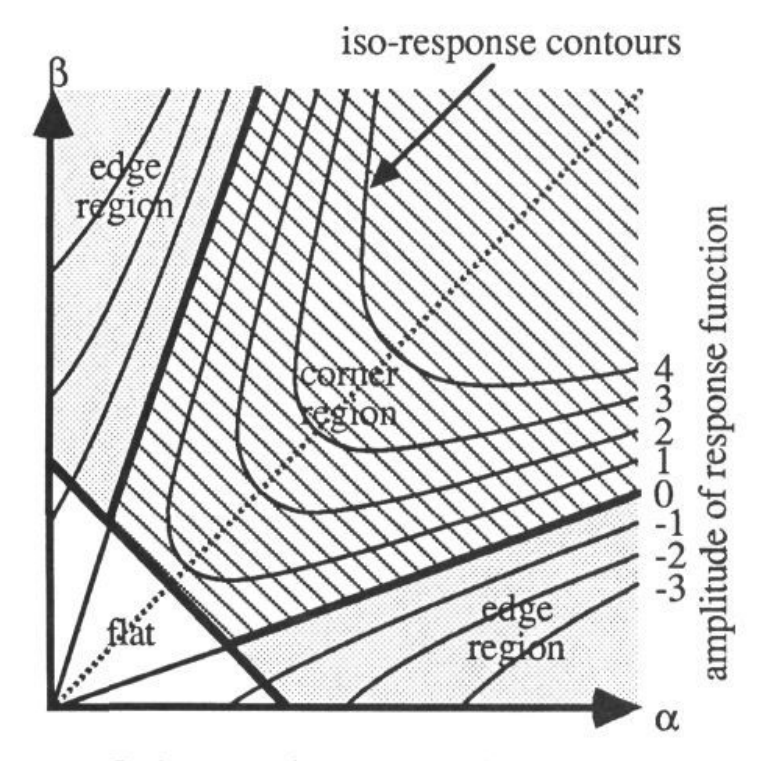
\includegraphics[height=0.25\pdfpageheight]{../Images/structure_tensor.png}
    \caption{Visualisation of distinction of image features using the eigenvalues of the structure
        tensor. $\alpha, \beta$ are equivalent to the eigenvalues $\lambda_1, \lambda_2$. Source: \cite{harris88}}\label{fig:Structure}
\end{figure}
There are different approaches to finding out whether the current location is a corner or an edge. The
simplest looking approach simply thresholds the smaller eigenvalue against some artificial
threshold. The set of local maxima is then the set of corners for the image\cite{shitomasi94}.
\TODO{Find sources for Rohr and Förstner}
However, this approach requires to compute both eigenvalues and can thus be fairly expensive.\\
A cheaper approach would be to either threshold the trace \[tr(\mathbf{J}_\rho) := j_{1, 1} + j_{2,
        2} = \lambda_1 + \lambda_2\] as proposed by Rohr, 1987 or the determinant \[det(\mathbf{J}_\rho) := j_{1, 1}j_{2, 2} -
    j_{1, 2}^2 = \lambda_1\lambda_2\] as proposed by Harris and F\"orstner, 1988 and 1986
respectively\cite{harris88}. Both of these approaches do not need to explicitly compute the eigenvalues of
the structure tensor and are thus not as computationally invested. The differences between the
approaches is that the first one requires the trace by itself to be a local maximum whereas in the
second approach, $\frac{det(\mathbf{J}_\rho)}{tr(\mathbf{J}_\rho)}$ needs to be a local maximum.\\

For the detection of relevant corners in the data selection phase, I mainly used the approach of F\"orstner/Harris as well as
the approach of Rohr even though the Tomasi-Kanade approach was an option and has also been
tested as we will see later in chapter \ref{ch:Results}. However, it has not proven as successful
as the other two methods during the initial testing phase.
\section{Diffusion}\label{sec:Diffusion}
\subsection{What is Diffusion?}
\subsection{Linear Diffusion}
\subsection{Nonlinear Diffusion}\label{sub:NonlinearDiff}
\section{Basics of Inpainting}\label{sec:Inpainting}
\subsection{EED-based Inpainting}
